\chapter{Suggested Solution}

\section{Architecture}\label{architecture}
\todo{Reword so it fits into the thesis. Change all links to github issues
to point to other sections of the thesis.}

We're using the redux-architecture for the won-owner-webapp javascript-client.
The architecture is strongly based on
\fnurl{http://redux.js.org/}{redux} in general and
\fnurl{https://github.com/wbuchwalter/ng-redux}{ng-redux} in particular. You can
find a short overview over these and their actions, reducers, the store and components
in section \ref{ref:redux}. For more in-depth
and hands-on documentation beyond what has been used for the work preceding
this thesis, I can recommend reading their well-done documentations.

So, this section will document in what ways our architecture diverges from or
builds on top of basic (ng-)redux, as well as list experiences and
style-recommendations from using it. %TODO these latter points should be in the critical reflection section

\begin{figure*}
\centering
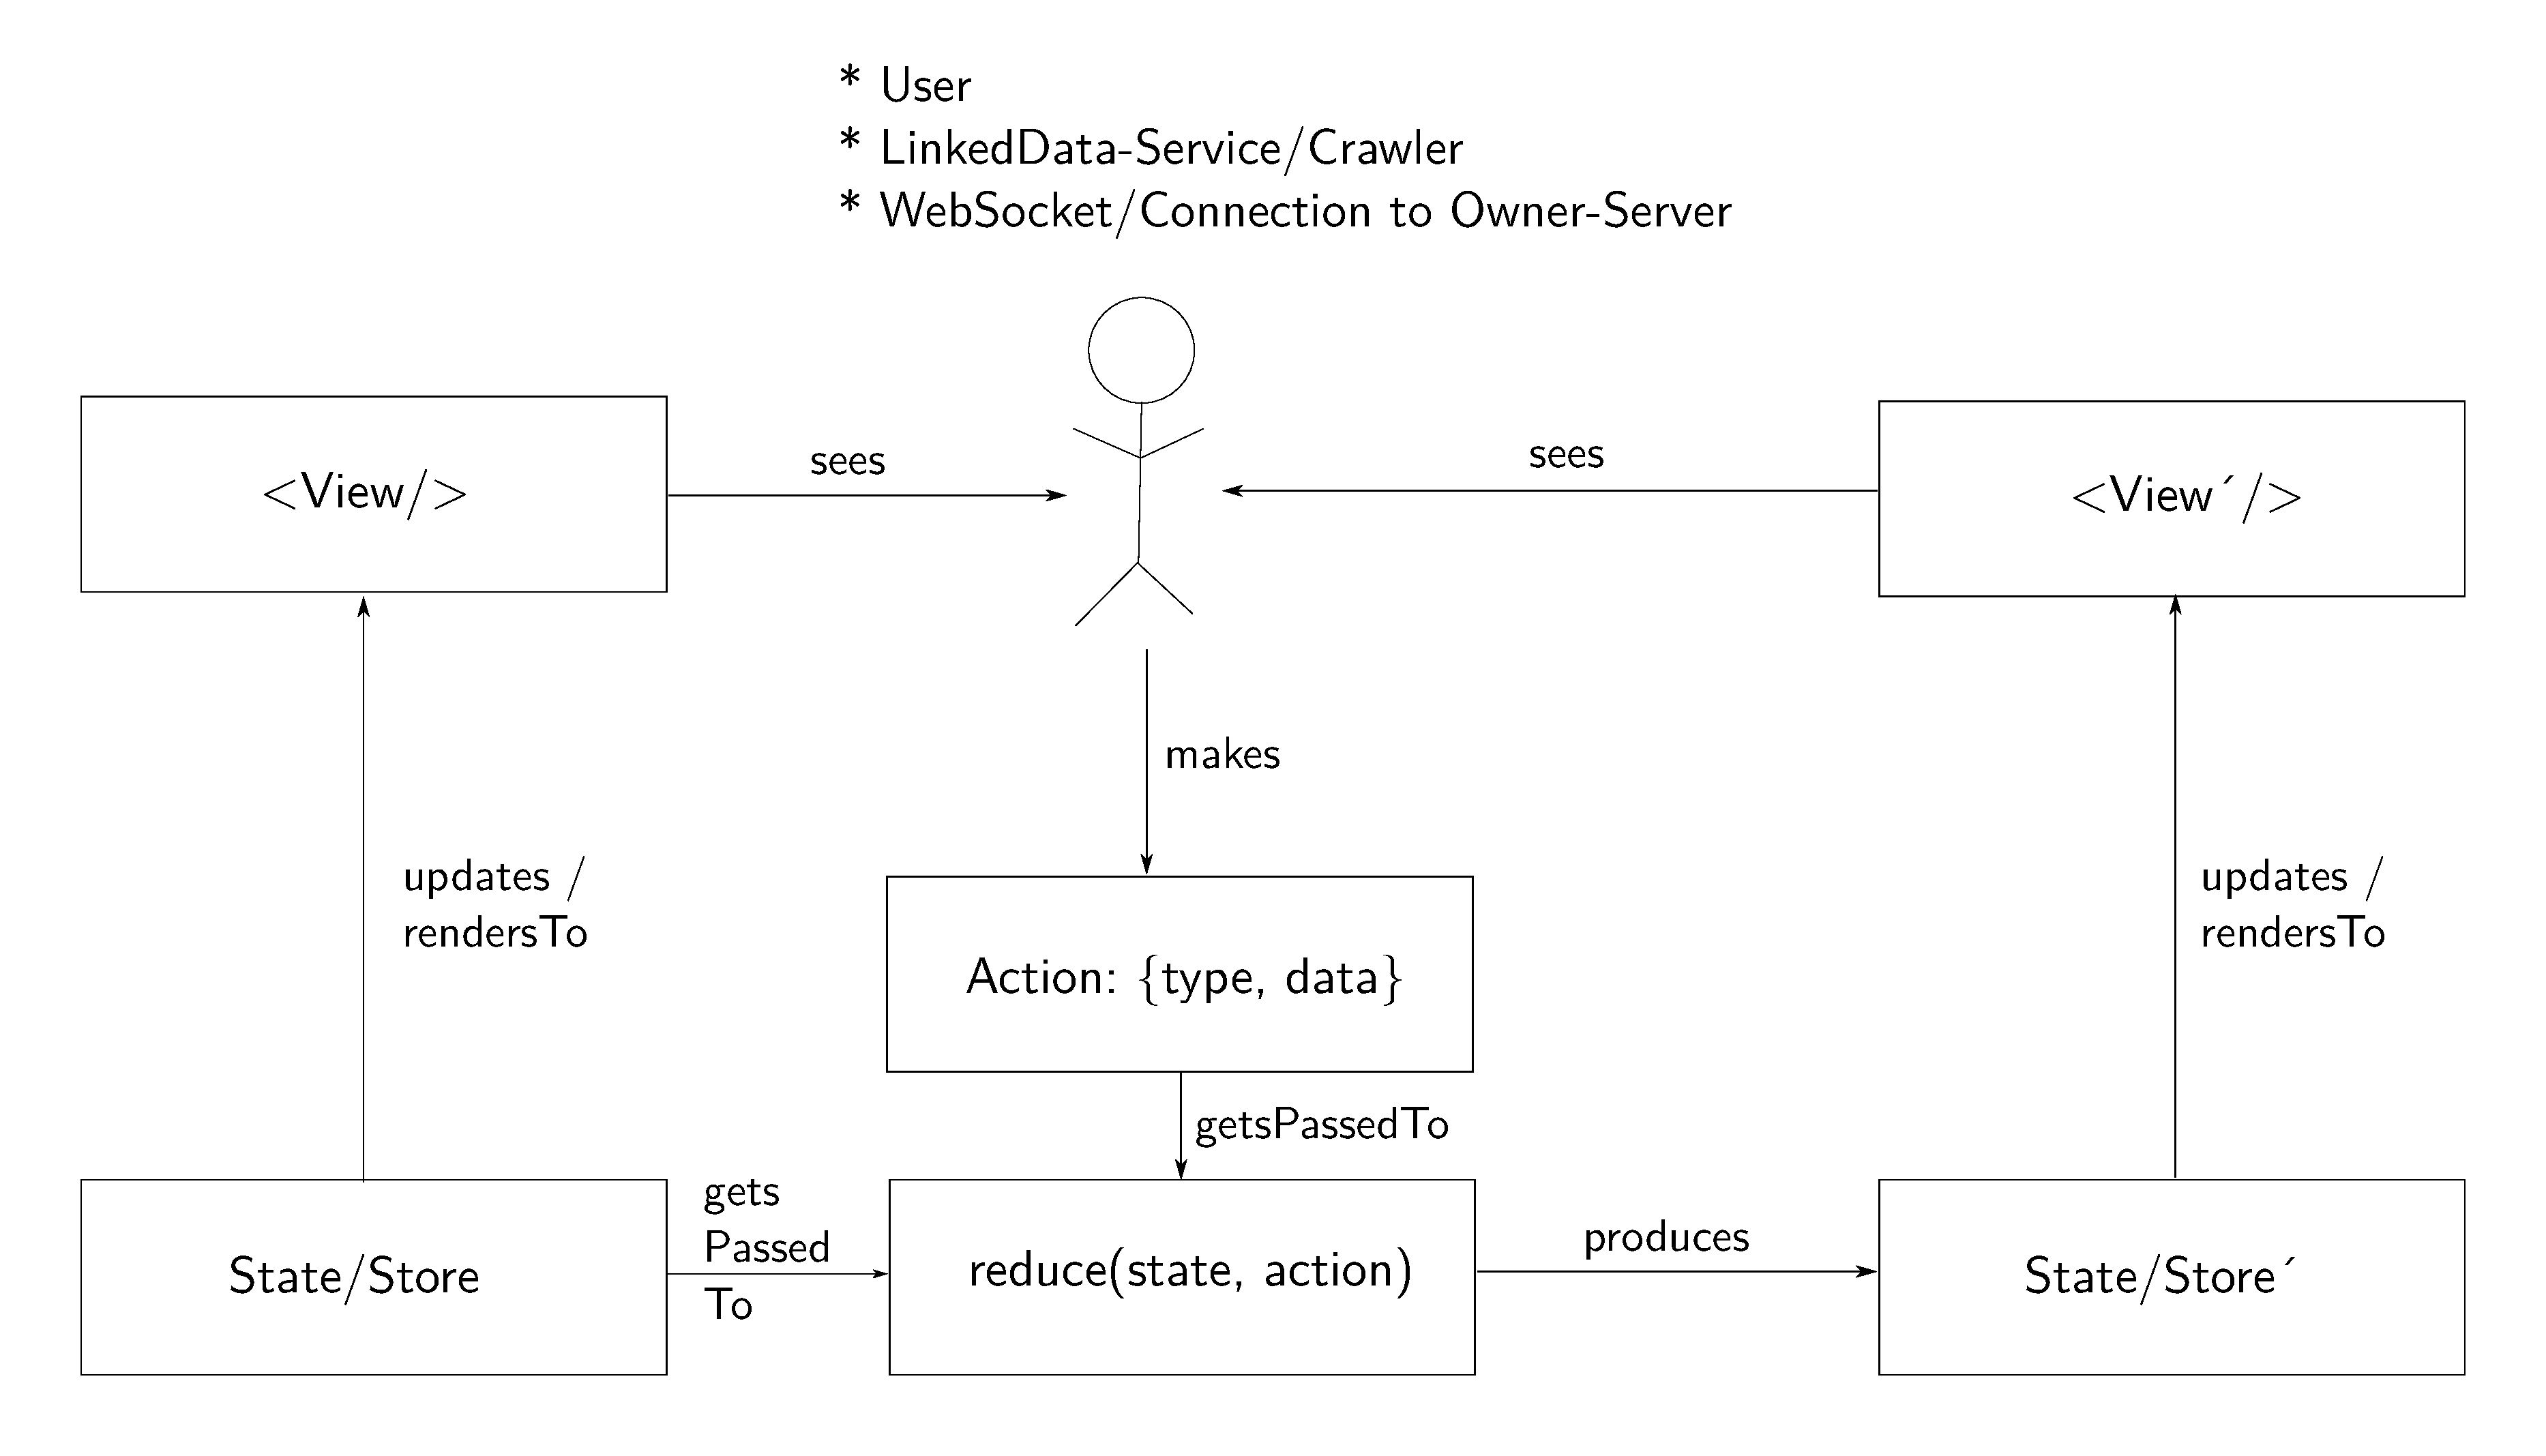
\includegraphics[width=1.0\textwidth]{figures/owner_app_redux_architecture.pdf}
\caption{\label{fig:adapted-redux}redux architecture in client-side owner-app}
\end{figure*}

\subsection{Action Creators}\label{sct:action-creators}

Can be found in \texttt{app/actions/actions.js} % TODO put into apendix

Anything that can cause \textbf{side-effects} or is
\textbf{asynchronous} should happen in these (tough they can also
be synchronous -- see \texttt{INJ\_DEFAULT}) %TODO code snippet
They should only be triggered
by either the user or a push from the server via the
\texttt{messagingAgent.js}. In both cases they cause a
\textbf{single}(!) action to be dispatched and thus passed as
input to the reducer-function.

If you want to \textbf{add new action-creators} do so by adding to the
\texttt{actionHierarchy}-object in \texttt{actions.js}. % TODO reword. this thesis isn't for colleagues working on the same code-base
From that two objects are generated at the moment:

\begin{itemize}
\tightlist
\item
  \texttt{actionTypes}, which contains string-constants

  (e.g.
  \texttt{actionTypes.drafts.change.title\ ===\
  \textquotesingle{}drafts.change.title\textquotesingle{}})
\item
  \texttt{actionCreators}, which houses the action creators. for the
  sake of injecting them with ng-redux, they are organised with
  \texttt{\_\_} as seperator (e.g.

  \texttt{actionCreators.drafts\_\_change\_\_title(\textquotesingle{}some\ title\textquotesingle{})})
\end{itemize}

Btw, the easiest way for actions without sideffects is to just placing
an \texttt{myAction:\ INJ\_DEFAULT}. This results in an action-creator
that just dispatches all function-arguments as payload, i.e.
\texttt{actionCreators.myAction\ =\ argument\ =\textgreater{}\ (\{type:\ \textquotesingle{}myAction\textquotesingle{},\ payload:\ argument\})}

Actions and their creators should always be describe \textbf{high-level user
stories/interactions} like \texttt{matches.receivedNew} or \texttt{publishPost}
(as opposed to something like \texttt{matches.add}
or \texttt{data.set})
Action-creators
encapsule all sideeffectful computation, as opposed to the reducers
which (within the limits of javascript) are guaranteed to be
side-effect-free. Thus we should do \textbf{as much as possible within
the reducers}. This decreases the suprise-factor/coupling/bug-proneness
of our code and increases its maintainability.

\subsection{Actions}\label{actions}

Can be found in \texttt{app/reducers/reducers.js} % TODO put into appendix

They are objects like
\texttt{\{type:\ \textquotesingle{}drafts.change.title\textquotesingle{},\ payload:\ \textquotesingle{}some\ title\textquotesingle{}\}}
and serve as input for the reducers.

See:
\href{https://github.com/researchstudio-sat/webofneeds/issues/342}{Actions/Stores
and Synching} %TODO should be in-thesis ref

\subsection{Reducers}\label{reducers}

Can be found in \texttt{app/reducers/reducers.js} % TODO put into appendix

These are \textbf{side-effect-free}. Thus as much of the implementation
as possible should be here instead of in the action-creators
to profit from this guarantee and steer clear of possible sources for
bugs that are hard to track down.

See ``Action Creators'' in section \ref{sct:action-creators} above for more detail

\subsection{Components}\label{components}

They live in \texttt{app/components/}. % TODO put into appendix?

Top-level components (views in the angular-sense) have their own folders
(e.g. \texttt{app/components/create-need/} and are split in two files).
You'll need to add them to the routing (see below) to be able to switch
the routing-state to these.

Non-top-level components are implemented as directives.

In both cases open up the latest implemented component and use the
boilerplate from these, if you want to implement your own. Once a
refined/stable boilerplate version has emerged, it should be documented
here.

\subsection{Routing}\label{routing}

We use
\href{https://github.com/angular-ui/ui-router/wiki/Quick-Reference}{ui-router}
and in particular the
\href{https://github.com/neilff/redux-ui-router}{redux-wrapper for it}
%TODO make thesis-intern

Routing(-states, aka URLs) are configured in \texttt{configRouting.js}. %TODO put into appendix
State changes can be triggered via
\texttt{actionCreators.router\_\_stateGo(stateName)}. % TODO too code-docu-like
The current
routing-state and -parameters can be found in our app-state:

\begin{verbatim}
$ngRedux.getState().get('router')
/* =>
{
  currentParams: {...},
  currentState: {...},
  prevParams: {...},
  prevState: {...}
}
*/
\end{verbatim}

Also see:
\href{https://github.com/researchstudio-sat/webofneeds/issues/344}{Routing
and Redux} %TODO make thesis-intern

\subsection{Server-Interaction}\label{server-interaction}

If it's \textbf{REST}-style, just use
\texttt{fetch(...).then(...dispatch...)} in an action-creator.
%TODO reword and elaborate

If it's \textbf{linked-data-related}, use the utilities in
\texttt{linkeddata-service-won.js}. They'll do standard HTTP(S) but will
make sure to cache as much as possible via the local triplestore.
%TODO reword and elaborate

If needs to \textbf{push to the web-socket}, add a hook for the
respective \emph{user(!)}-action in \texttt{message-reducers.js}. The
\texttt{messaging-agent.js} will pick up any messages in
\texttt{\$ngRedux.getState().getIn({[\textquotesingle{}messages\textquotesingle{},
\textquotesingle{}enqueued\textquotesingle{}  ]})}
and push them to it's websocket. This solution appears rather hacky to
me (see `high-level interactions' under `Action Creators') and I'd be
thrilled to hear any alternative solutions :)
%TODO reword and elaborate

If you want to \textbf{receive stuff the web-socket}, go to
\texttt{actions.js} and add your handlers to the
\texttt{messages\_\_messageReceived}-actioncreator. The same I said
about pushing to the web-socket also holds here.
%TODO reword and elaborate

\section{Tooling}\label{tooling}

\begin{comment}
See:

\begin{itemize}
\tightlist
\item
  \href{https://github.com/researchstudio-sat/webofneeds/issues/300}{Angular
  2.0} -\textgreater{} it wasn't ready at the time of the decision
\item
  \href{https://github.com/researchstudio-sat/webofneeds/issues/314}{Precompilation
  and Tooling (Bundling, CSS, ES6)}
\end{itemize}
\end{comment}
